% Source: AESP_466_ClassWork/Assignments/Assignment_1/AESP466_HW1_Solutions_Sp26.tex
% Description: Pendulum with Torsional Spring Configuration

\documentclass[border=4pt]{standalone}
\usepackage{amsmath}
\usepackage{amssymb}
\usepackage{graphicx}
\usepackage{tikz}
\usepackage{xcolor}
\usetikzlibrary{arrows.meta, calc, patterns, angles, quotes, 3d, decorations.pathmorphing}

\definecolor{Garnet}{HTML}{73000A}
\definecolor{USC_Rose}{HTML}{CC2E40}
\definecolor{USC_Blue}{HTML}{466A9F}
\definecolor{USC_Slate}{HTML}{1F414D}
\definecolor{USC_Olive}{HTML}{65780B}
\definecolor{USC_Lime}{HTML}{CED318}
\definecolor{USC_Gold}{HTML}{A49137}
\definecolor{USC_Black90}{HTML}{565656}
\definecolor{USC_Black10}{HTML}{ECECEC}

\begin{document}
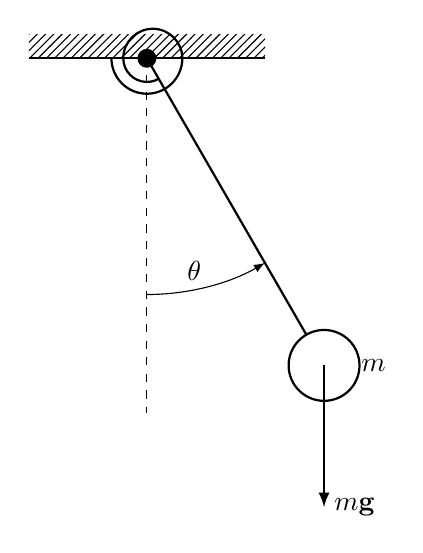
\begin{tikzpicture}[scale=1.5, >=latex]
    % Ceiling / Support
    \fill[pattern=north east lines] (-1,0) rectangle (1,0.2);
    \draw[thick] (-1,0) -- (1,0);

    % Vertical Reference Line
    \draw[dashed] (0,0) -- (0,-3);

    % Rod
    \draw[thick] (0,0) -- (1.5,-2.6);

    % Torsional Spring (Spiral)
    \draw[thick] (-0.3, 0)
        arc (180:360:0.3)
        arc (0:180:0.25)
        arc (180:300:0.2) -- (0.1, -0.173);

    % Pivot Point
    \fill[black] (0,0) circle (0.08);

    % Mass (Circle with white fill)
    \filldraw[fill=white, thick] (1.5,-2.6) circle (0.3);
    \node[right=0.35cm] at (1.5,-2.6) {$m$};

    % Angle Theta
    \draw[->] (0,-2) arc (-90:-60:2);
    \node at (0.4,-1.8) {$\theta$};

    % Gravity
    \draw[->, thick] (1.5,-2.6) -- (1.5,-3.8) node[right] {$m\mathbf{g}$};
\end{tikzpicture}
\end{document}
